%% ----------------------------------------------------------------
%% Chapter 5: A machine-learning model for SANS
%% ----------------------------------------------------------------
%!TeX root = subfile
\label{chapter:zanspy}
\documentclass[../main.tex]{subfiles}
% ---------------------------------------------------------------- 
\begin{document}

The modelling of the SANS closure terms is critical for the prediction of 3-D spanwise-averaged dynamics in 2-D systems.
An standard EVM, such as the Smagorinsky model, has failed to correctly predict the SANS closure terms because of if intrinsic dissipative and linear behaviour.
While other physical models allowing energy backscatter (energy transfer from small to large scales) such as the dynamic Smagorinsky model or a transport equation model could be explored in the future, in this chapter a data-driven model is proposed.
The limited knowledge on the spanwise stresses dynamics motivates this choice.
In particular, a supervised machine-learning (ML) model based on a deep convolutional neural network has been designed for this purpose.
A-priori results show up to 92\% correlation between target and predicted closure terms; more than an order of magnitude better than the EVM correlation.
Additionally, the ML model performance is assessed for a different flow configuration (Reynolds regime and body shape) to the training case and high correlation values are still captured.
The new SANS equations and ML closure model are also used for a-posteriori prediction.
Even though evidence of known stability issues with long-time ML predictions for dynamical systems is found for the present data-driven model, the closed SANS simulations are still capable of predicting wake metrics and induced forces with errors from 1-10\%.
This results in approximately an order of magnitude improvement over standard 2-D simulations while reducing the computational cost of 3-D simulations by 99.5\%.

\section{Introduction and literature review}

In recent years, machine learning, i.e. algorithms that reveal information by processing raw data inputs, have made an impact across numerous disciplines: from image recognition, to improved web searches, content filtering, natural language processing, among others \citep{LeCun2015}.
The fluid mechanics community has also adopted ML techniques both in experimental and computational work, specifically with the use of deep-learning methods \citep{Kutz2017}, where multiple layers of trainable parameters are stacked sequentially.
As data-driven models learn from observations, the vast amounts of data generated through field measurements and high-fidelity simulations has accelerated the application of ML models to fluid flow problems \citep{Brunton2020}. 

Supervised learning, or model optimisation based on labelled examples, has yielded the exploration of novel flow classification, control, and regression techniques.
Within classification and uncertainty quantification, detection of low RANS accuracy regions in the flow has been accomplished with the use of different ML strategies such as support vector machines and random trees \citep{Ling2015}.
Deep artificial neural networks (ANNs) have been employed for uncertainty quantification in RANS \citep{Geneva2019}, pointwise classification and blending of appropriate turbulence closures in LES \citep{Maulik2019}, and discovery of active flow control strategies such as drag reduction in turbulent channel flow \citep{Lee1997}.

Different control strategies have been developed using reinforcement learning which, in contrast to supervised learning, does not rely in labelled examples and the algorithm objective is to maximise a long-term reward signal based on self-proposed actions \citep{SuttonBarto2018}. 
Reinforcement learning has been used for (e.g.) active wake flow control \citep{Rabault2019a,Rabault2019b} and efficient control of collective swimmers \citep{Verma2018}.
Other unsupervised learning models such as generative adversarial networks \citep{Goodfellow2014} have been used for unsteady flow field generation \citep{Lee2019}.

The use of ML models for regression problems in fluid flows has also bloomed in the last few years. ANNs have been used for the reconstruction of turbulent spatio-temporal sampled data \citep{Deng2019}, physics-based discovery of governing equations parameters such as Reynolds number \citep{Raissi2019}, quantitative prediction of flow fields from scalar concentration snapshots \citep{Raissi2020}, and RANS modelling \citep{Duraisamy2015,Ling2016,Lapeyre2019}, among others.
Convolutional neural networks (CNNs) have also become a popular tool to solve regression problems.
CNNs have been used for turbulent flow field super-resolution \citep{Fukami2019,Liu2020}, modelling of surface pressure distribution from sparse wake flow data \citep{Ye2020}, nonlinear mode decomposition \citep{Murata2019}, and prediction of turbulent fields \citep{Lapeyre2019,Kim2020b,Kim2020a}, among others. 

Specifically within turbulence closures, CNNs have been applied in RANS \citep{Weatheritt2016} and LES \citep{Gamahara2017,Beck2019} frameworks, establishing its utility for revealing hidden correlations between system variables for which physical laws are, a-priori, unknown \citep{Brenner2019}.
In particular, CNNs have been developed to efficiently learn spatial structures in data arrays by exploiting the translational invariance inherent in convolutions \citep{LeCun1995}.
This makes them a very attractive tool for modelling novel and spatially-complex fields such as the new SANS closures.

With respect to the strip-based SANS framework, the general methodology of the data-driven ML model is based on the idea that training a SANS closure on a single local spanwise segment (see \fref{fig:strips}) automatically generalises to all the spanwise-averaged strips because of the system homogeneity in that direction.
Hence, the database required to train the model can be generated in a single 3-D simulation with a span equivalent to the local spanwise-averaging length.
For example, a structure of aspect ratio 100 can be reduced to 100 strips, or 2-D simulations, resolving the (1-diameter) SANS equations.
The required SANS closure model can be previously trained using data of a 3-D high-fidelity simulation of a 1-diameter-long spanwise-periodic cylinder, noting that the 3-D simulation is the most computationally expensive part of the method as detailed in \aref{chapter:appendixE}.
In this chapter, the ML SANS closure model is assessed for a single spanwise-averaged strip of 1 diameter.

\section{Machine-learning model} \label{sec:ML_model}

Data-driven closures are particularly helpful when physical information of the system to be modelled is not known a-priori, and this is certainly the case for the novel spanwise stresses developed in this work.
Hence, in this section we present a ML model for the spanwise fluctuations thus providing closure to the SANS equations.

A CNN is proposed to map resolved quantities, $\mathrm{X}_n=\left\lbrace U,V,P\right\rbrace$, to closure terms, $\mathrm{Y}_n$.
The CNN architecture is depicted in \fref{fig:cnn2}.
The closure terms of the a-priori analysis are the SSR tensor components (similarly to \sref{sec:evm}), $\mathrm{Y}_n=\left\lbrace \avg{u\p u\p},\avg{u\p v\p},\avg{v\p v\p}\right\rbrace$.
On the other hand, the perfect closure is targeted as the output of the a-posteriori analysis, $\mathrm{Y}_n=\lbrace \mathcal{S}^R_x,\mathcal{S}^R_y\rbrace$, in order to improve the model stability as will be discussed in \sref{sec:ML_a-post}.

The ML model architecture is based on a multiple-input multiple-output CNN (MIMO-CNN). 
The need of a high-dimensional tunable function that can reveal hidden correlations in spatial data motivates the CNN choice \citep{LeCun1989}.
The same model architecture is used for both a-priori and a-posteriori analysis, where only the number of outputs changes from three to two, respectively.
Each input branch is composed of an encoding part and a decoding part.
The number of filters doubles at every convolutional layer in the encoding part, reaching a maximum of 64 filters, and halves in the decoding part.
Each convolutional layer consists of a 2-D convolution operation with a $5\times5$ filter (convolution kernel), a batch normalisation operation, and a rectified linear unit (ReLU) activation function.
The total number of trainable parameters is 944,739.
The batch normalisation helps to speed up the neural network learning rate and improves its stability with respect to the random weights initialisation \citep{Ioffe2015}. 
The ReLU function allows higher learning rates and handles vanishing-gradient problems better than other standard activation functions such as the Sigmoid or the $\tanh$ functions \citep{Nair2010}.
All input branches are then concatenated into a single branch, for which another encoding-decoding branch follows.
The last layer consists of a wake mask function and a Gaussian filter.

The wake mask helps providing a clean output in the regions of the domain where the closure terms are negligible.
The wake mask is based in the vorticity field for which the condition $|\Omega_z|>\epsilon$ is applied.
Hence, a field of 1s (and 0s) is generated when the condition is met (or not).
The wake mask for the a-priori stage considers all the points within the wake limit.
The wake limit is activated using the $\epsilon=1\cdot10^{-3}$ threshold (\fref{fig:wake1}).
This helps the model focusing on the non-trivial region during optimisation while still providing some areas within the wake width where the closure term is not active.
The wake mask for the a-posteriori stage applies the criterion in a pointwise manner, hence points within the wake region might not be activated, particularity in the far wake region (\fref{fig:wake2}).
Also, the criterion is more strict by setting $\epsilon=3.5\cdot10^{-3}$.
This is enforced to improve the stability of the a-posteriori analysis so longer temporal dynamics can be evaluated.
Finally, a Gaussian filter of $\sigma=0.5$ (resulting in a $5\times5$ kernel matching the feature maps size) is applied to the output of the wake detection layer.

\begin{figure}[t]
\centering
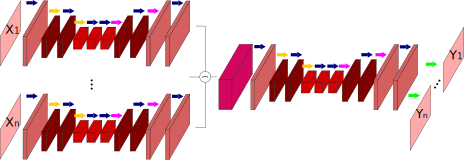
\includegraphics[width=0.95\linewidth]{chapter5/cnn/cnn}\vspace{-0.1cm}
\caption{CNN architecture.
An encoding-decoding branch is considered for each input field.
The input branches are then concatenated $(\frown)$ and another encoding-decoding branch follows.
The closure terms are separately extracted on the last layer.
Arrows legend: Dark blue: Conv2D $5\times5$ $+$ batch normalisation $+$ activation function.
Yellow: MaxPooling $2\times2$.
Magenta: UpSampling $2\times2$.
Green: Conv2D $1\times1$ $+$ wake mask $+$ Gaussian filter.
Block thickness indicates the number of filters, which double/halve at each convolutional operation in the encoding/decoding parts.}
\label{fig:cnn2}
\end{figure}

\begin{figure}[!ht]
\centering
\begin{subfigure}{0.7\linewidth}
 	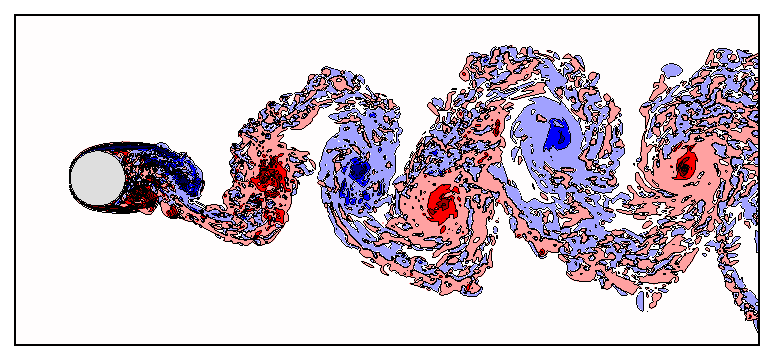
\includegraphics[width=\linewidth]{chapter5/wake/vort}
 	\caption{$\Omega_z$} 
\end{subfigure}
\begin{subfigure}{0.7\linewidth}
    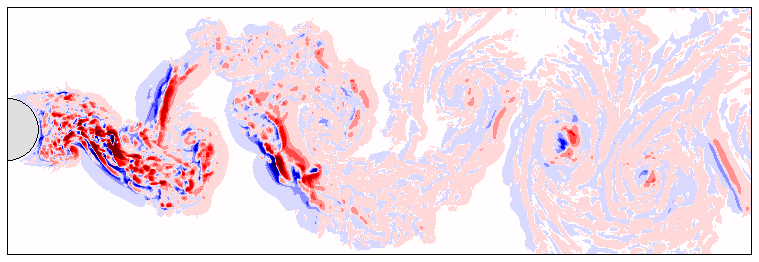
\includegraphics[width=\linewidth]{chapter5/wake/SRx}
	\caption{$\mathcal{S}^R_x$}
\end{subfigure}
\begin{subfigure}{0.7\linewidth}
	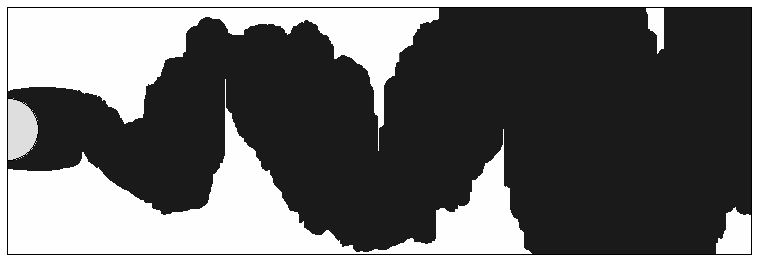
\includegraphics[width=\linewidth]{chapter5/wake/wake1}
	\caption{Wake mask used in the a-priori analysis.}\label{fig:wake1}
\end{subfigure}
\begin{subfigure}{0.7\linewidth}
	\includegraphics[width=\linewidth]{chapter5/wake/wake2} 
	\caption{Wake mask used in the a-posteriori analysis.}\label{fig:wake2}
\end{subfigure}
\caption{A wake mask from the vorticity field is generated to focus the ML model outputs on the non-trivial wake region alone. The aim is to match the region where the target output $(\mathcal{S}^R_x)$ is activated. In the a-posteriori analysis, the far-wake region is not fully activated in order to aid the closure stability.}
\end{figure}

A detailed hyper-parametric study of the ML model has been conducted for the circular cylinder case (similarly to \sref{sec:SANS_circular_cylinder}) in \cite{Font2020a}, and is also included in \aref{chapter:appendixD}.
In short, the present model architecture was compared against two different MIMO-CNNs, and this architecture offered the best accuracy among the tested models.
Also, it was found that the larger the CNN (in terms of trainable parameters), the faster high correlation coefficients were obtained for a similar number of training epochs (where epoch refers to an optimisation iteration on the training dataset).
The number of trainable parameters was modified by changing the number of filters per layer.
The sum of the squared error as a loss function provided the best performance when compared to the sum of the absolute error.
The use of primitive variables (velocity and pressure) did not yield significant differences when compared to the velocity gradient tensor components set. 
Both these input sets showed a better performance than a third input set containing the vorticity field and the distance function to the cylinder.

Unsteady turbulent flow past a circular cylinder with a 1 diameter span $(L_z=1)$ at $Re=10^4$ (as considered in \sref{sec:SANS_circular_cylinder}) has been used to generate a dataset containing a total of 7000 samples of $1216\times540$ size during $\Delta t^*=1650$ and using a sampling rate of $\delta t^*=0.25$.
The 1 diameter span is sufficiently long to sustain 3-D turbulence on a meaningful wake region and it is also a sensible choice of the minimum structural mode wavelength that would need to be resolved in a SANS-based strip-theory framework.
The input fields are normalised with the standard score, i.e. $\hat{x} = (x-\overline{x})/\sigma_x$.
As in \cite{Beck2019, Kim2020a}, a single $Re$ regime is used in the dataset generation, which is deemed sufficient because of the turbulent nature and unsteadiness of the flow.
The constant energy transfer rate across different scales in the inertial subrange of turbulence implies that closures trained on one $Re$ should generalise reasonably well to unseen $Re$ as long as the mean flow characteristics are similar.
Such study is conducted in \sref{sec:generalisation}.

The dataset is split with 6000 samples for optimisation (training), 500 samples for validation during training, and 500 for evaluation (testing) purposes.
The dataset split is chosen as often encountered in the machine learning literature, probably adopted from power law (or Pareto) distributions \citep{Newman2005}.
To ensure the closure's ability to generalise and avoid overfitting, the time windows for testing, optimisation and validation do not overlap, i.e. the closure is assessed on a continuous window of previously unseen flow.
A mini-batch stochastic gradient descent method based on the Adam optimiser \citep{Kingma2014} is used to update the network weights during training.
The sum of the squared error function is used for optimisation
\begin{equation}
\mathrm{Loss}=\sum^m_i\sum^n_j \pars{\mathrm{Y}_{i,j}-\mathrm{Y}_{i,j}^{\mathrm{ML}}}^2,
\end{equation}
where $m$ is the size (number of samples) of the mini-batch, $n$ is the output index, and the superscript $(\cdot)^{\mathrm{ML}}$ denotes the ML model prediction.
When the validation error does not decrease for 5 epochs or a total of 60 epochs is reached, training is stopped (a.k.a. early-stopping).

\begin{figure}[!t]
\setlength{\columnsep}{-1pt} 
\begin{multicols}{2}
\centering
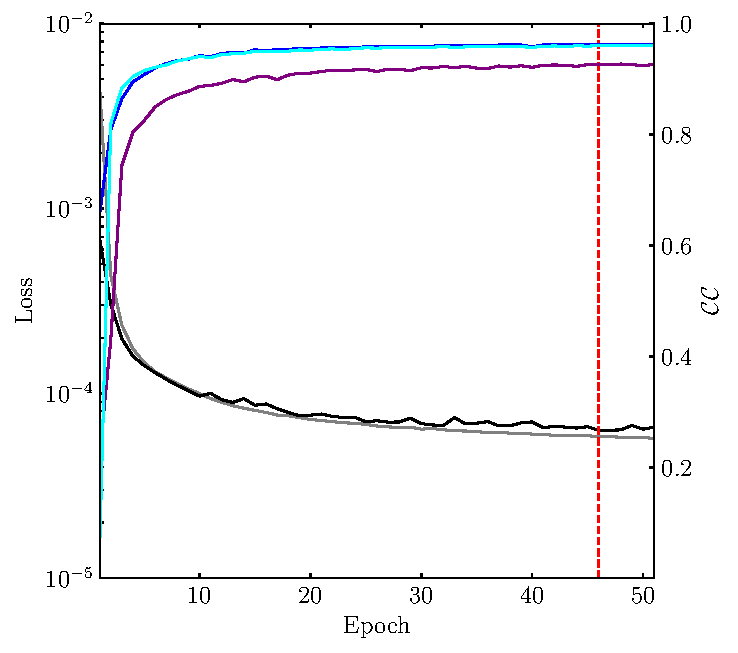
\includegraphics[width=1.02\linewidth]{chapter5/a-priori/history_ab}
\caption{Training of the $\mathrm{Y}_n=\big\lbrace\langle u' u'\rangle,\langle u' v'\rangle,\langle v' v'\rangle\big\rbrace$ output set.
The vertical red dashed line indicates the early stop.
Grey: combined training loss.
Black: combined validation loss.
Blue: $\langle u' u'\rangle$ correlation coefficient.
Purple: $\langle u' v'\rangle$ correlation coefficient.
Cyan: $\langle v' v'\rangle$ correlation coefficient.}\label{fig:ab_history}

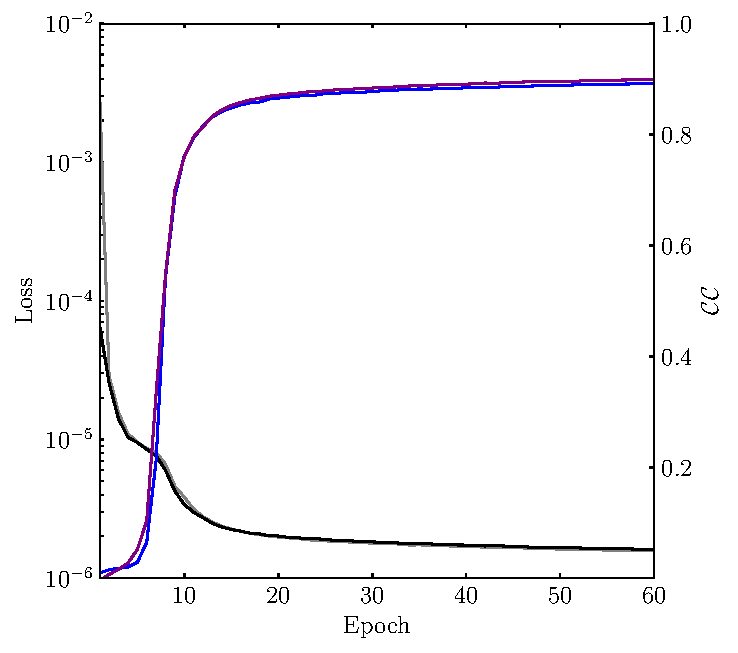
\includegraphics[width=1.02\linewidth]{chapter5/a-priori/history_SR}
\caption{Training of the $\mathrm{Y}_n=\big\lbrace \mathcal{S}^R_x, \mathcal{S}^R_y \big\rbrace$ output set.
Grey: combined training loss.
Black: combined validation loss.
Blue: $\mathcal{S}^R_x$ correlation coefficient.
Purple: $\mathcal{S}^R_y$ correlation coefficient.}
\label{fig:SR_history}
\end{multicols}
\end{figure}

The ML model training history of the SSR tensor components is plotted in \fref{fig:ab_history}, where a rapid convergence cap be appreciated.
The early-stopping criterion is triggered on the 46th epoch since it provides the lowest validation error not improved for the next 5 epochs.
On the other hand, the training history of the perfect closure components is plotted in \fref{fig:SR_history}.
In this case, the early-stopping criterion is not triggered and optimisation is performed during 60 epochs (the maximum defined).

\section{Results}

\subsection{A-priori analysis}

To allow a comparison with the EVM, the anisotropic part of the SSR tensor is recovered from the ML model predictions of the full SSR tensor.
The fact that the ML model yields the full SSR tensor already provides an advantage with respect to the EVM since no further modifications of the governing equations are required, nor an additional transport equation for the SSR kinetic energy.

The predicted anisotropic SSR tensor components $(\boldsymbol\tau^{r,\,\mathrm{ML}}_{11}, \boldsymbol\tau^{r,\,\mathrm{ML}}_{12}, \boldsymbol\tau^{r,\,\mathrm{ML}}_{22})$ are depicted in \fref{fig:ML_a-priori}, and the predicted components of the full SSR tensor $(\avg{u\p u\p}^{\mathrm{ML}}, \avg{v\p v\p}^{\mathrm{ML}})$ are depicted in \fref{fig:ML_ab_a-priori}.
It can be appreciated that large-scale structures are overall correctly captured.
On the other hand, small-scale structures, such as those encountered in near-wake region, are more difficult to predict.
Similar issues have been found for other CNN-based data-driven models \citep{Lee2019}.
A Gaussian filtering operation together with a wake detection feature aids the CNN to provide less noisy predictions focused on the wake region alone.
This helps mitigating error propagation in an a-posteriori framework (see next section), however, it can have an impact on the small-scale structures as well.

A significant improvement is qualitatively observed when comparing the predictions against the EVM, where the latter fails to capture almost all flow structures except for the largest ones (\fref{fig:EVM_a-priori}).
Furthermore, correlation values above $90\%$ have been achieved for all the anisotropic SSR tensor components (\tref{tab:ML_a-priori}), as well as the full SSR tensor components (\tref{tab:ML_ab_a-priori}).
It can be concluded that the ML model provides a significantly better prediction of the closure terms compared to the EVM, which is critical for SANS to correctly model turbulence wake dynamics.

\begin{figure}[!ht]
\centering
\begin{subfigure}[t]{0.6\linewidth}
    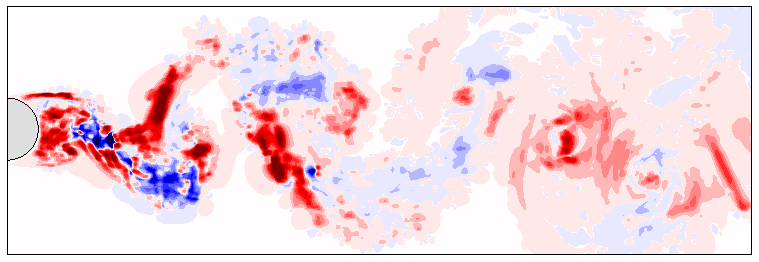
\includegraphics[width=\linewidth]{chapter5/a-priori/tau_r_11_lowres}
    \caption{$\boldsymbol\tau^r_{11}$} 
\end{subfigure}
\begin{subfigure}[t]{0.6\linewidth}
    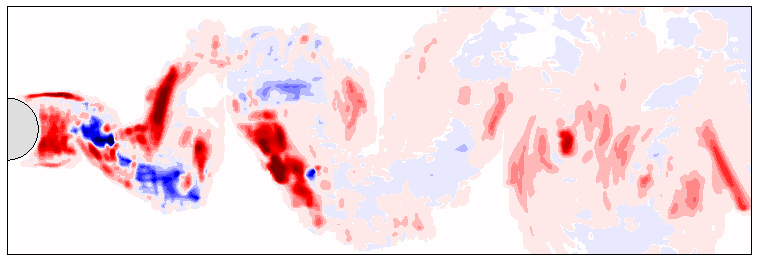
\includegraphics[width=\linewidth]{chapter5/a-priori/tau_r_11_ML_lowres}
    \caption{$\boldsymbol\tau^{r,\,\mathrm{ML}}_{11}$}
\end{subfigure}
\begin{subfigure}[t]{0.6\linewidth}
    \includegraphics[width=\linewidth]{chapter5/a-priori/tau_r_12_lowres}
    \caption{$\boldsymbol\tau^r_{12}$}
\end{subfigure}
\begin{subfigure}[t]{0.6\linewidth}
    \includegraphics[width=\linewidth]{chapter5/a-priori/tau_r_12_ML_lowres}
    \caption{$\boldsymbol\tau^{r,\,\mathrm{ML}}_{12}$}
\end{subfigure}
\begin{subfigure}[t]{0.6\linewidth}
    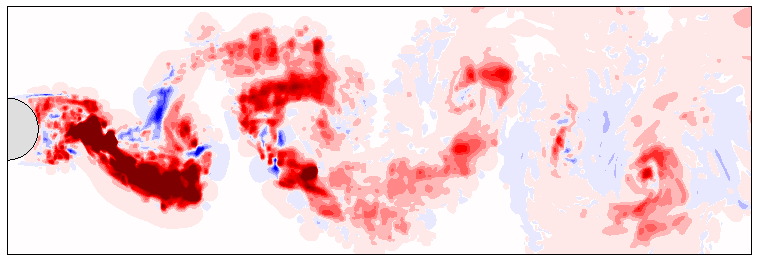
\includegraphics[width=\linewidth]{chapter5/a-priori/tau_r_22_lowres}
    \caption{$\boldsymbol\tau^r_{22}$}
\end{subfigure}
\begin{subfigure}[t]{0.6\linewidth}
    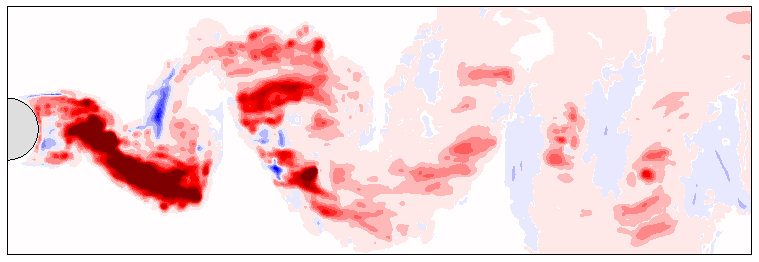
\includegraphics[width=\linewidth]{chapter5/a-priori/tau_r_22_ML_lowres}
    \caption{$\boldsymbol\tau^{r,\,\mathrm{ML}}_{22}$}
\end{subfigure}
\caption{ML model prediction of the anisotropic SSR tensor components compared to reference data.}
\label{fig:ML_a-priori}
\end{figure}

\begin{table}[t]
\centering
\caption{Correlation coefficients between components of the anisotropic SSR tensor and predictions provided by the EVM and the ML model.}
\begin{tabular}{lrrr}
\toprule
$\mathcal{CC}$ & $\boldsymbol\tau^r_{11}$ & $\boldsymbol\tau^r_{12}$ & $\boldsymbol\tau^r_{22}$ \\
\midrule
EVM &  0.06& 0.06 & 0.14\\
ML &  0.90   & 0.92 & 0.92\\
\bottomrule \label{tab:ML_a-priori}
\end{tabular}
\end{table}

\begin{table}[t]
\centering
\caption{Correlation coefficients between target SSR tensor components and ML model predictions.}
\begin{tabular}{lrrr}
\toprule
$\mathcal{CC}$ & $\avg{u\p u\p}$ & $\avg{u\p v\p}$ &$\avg{v\p v\p}$  \\
\midrule
ML & 0.95 & 0.92 & 0.96\\
\bottomrule \label{tab:ML_ab_a-priori}
\end{tabular}

{\footnotesize The correlation coefficients are calculated for the 500 snapshots of the test dataset and the average values are provided. \par}
\end{table}

\begin{figure}[!ht]
\centering
\begin{subfigure}[t]{0.6\linewidth}
    \includegraphics[width=\linewidth]{chapter5/a-priori/tau_R_11_lowres}
    \caption{$\avg{u\p u\p}$} 
\end{subfigure}
\begin{subfigure}[t]{0.6\linewidth}
    \includegraphics[width=\linewidth]{chapter5/a-priori/tau_R_11_ML_lowres}
    \caption{$\avg{u\p u\p}^{\mathrm{ML}}$}
\end{subfigure}
\begin{subfigure}[t]{0.6\linewidth}
    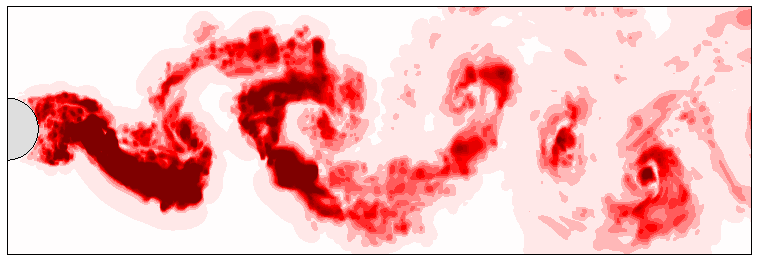
\includegraphics[width=\linewidth]{chapter5/a-priori/tau_R_22_lowres}
    \caption{$\avg{v\p v\p}$}
\end{subfigure}
\begin{subfigure}[t]{0.6\linewidth}
    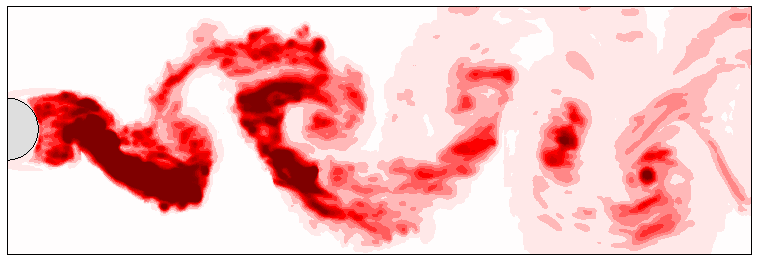
\includegraphics[width=\linewidth]{chapter5/a-priori/tau_R_22_ML_lowres}
    \caption{$\avg{v\p v\p}^{\mathrm{ML}}$}
\end{subfigure}
\caption{ML model prediction of the full SSR tensor components compared to reference data.}
\label{fig:ML_ab_a-priori}
\end{figure}

\clearpage

\subsection{Generalisation across flow regimes and geometries}\label{sec:generalisation}

So far, it has been demonstrated that the trained ML model can correctly predict the SANS closure terms of previously unseen snapshots of the cylinder case, i.e. the model has correctly generalised in time.
Here, the generalisation of the ML model to other flow configurations such as body shapes and Reynolds regimes is assessed.
This analysis is important because, first, it provides information on whether training the ML model in a fixed set-up can still be useful for the prediction of the SANS stresses in a different case.
Second, it is a good test to check that the ML model has not over-fitted the training data even with the use of the early-stopping criterion.

Four different cases are studied:
Flow past a circular cylinder at $Re=1000$.
Flow past a circular cylinder at $Re=3900$.
Flow past an ellipse with axis $(x,y)=(2D,D)$ (ellipse 1) at $Re=10^4$.
Flow past an ellipse with axis $(x,y)=(0.5D,D)$ (ellipse 2) at $Re=10^4$.
Similarly to the circular cylinder case at $Re=10^4$, a test dataset of 500 snapshots has been generated during $\Delta t^*=125$ time units after reaching a statistically stationary state of the wake for all cases.
Both output target sets, i.e. the full SSR tensor components and the perfect closure components, are analysed.

\tref{tab:ML_generalisation} quantifies the accuracy of the ML model in terms of mean correlation coefficient to target data. 
Note that correlation values are provided for two wake regions, and these can be visualized in \fref{fig:cc_regions}:
one involving the non-trivial wake region (same region as used in previous results, noted in green dashed lines) and one discarding the region surrounding the body (noted in blue dashed lines), i.e. $x\in[0.75D_x,12D_y]$ where $D_x$ and $D_y$ are the streamwise and crossflow body lengths, respectively.
With respect to the model generalisation in different Reynolds regimes, its prediction ability on the $Re=3900$ case is similar to the training case ($Re=10^4$) since the correlation values provided in both cases are very close.
For the $Re=1000$ case, similar results are also obtained to the training case, specially when the near-body region is cropped out of the correlation analysis.
Qualitatively, the ML model prediction of the spanwise stresses is displayed in \fref{fig:ML_generalisation_R1} and \fref{fig:ML_generalisation_R2} for the $Re=1000$ and $Re=3900$ cases, respectively.
Again, a similar performance to the training case is observed;
mid- and large-scale structures are correctly captured whereas small-scale structures are not reconstructed as in the target data.
For the $Re=1000$ case, it can also be observed how the ML model struggles to predict the spanwise stresses in the region near to the body.

\begin{figure}[t]
\centering
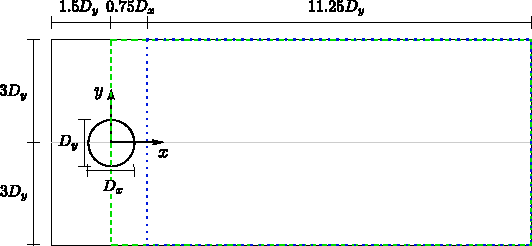
\includegraphics[width=0.75\linewidth]{chapter5/generalisation/cc_regions}
\caption{Regions used for the ML model analysis.
Black: Input and output region of the ML model. 
Green dashed: Region used to compute the correlation coefficient between ML predictions and target data (full wake).
Blue dotted: Region used to compute the correlation coefficient between ML predictions and target data omitting the near-body domain (downstream wake).}
\label{fig:cc_regions}
\end{figure}

Regarding the ellipse cases at $Re=10^4$, high correlation values are observed when the near-body region is cropped out of the correlation analysis as displayed \tref{tab:ML_generalisation}.
On the other hand, the ML model fails to correctly predict the spanwise stresses in the shear-layer region.
This behaviour can be appreciated in \fref{fig:ML_generalisation_E1} and \fref{fig:ML_generalisation_E2}, where patches of high-intensity spanwise stresses arise at the vicinity of the body.
To a lesser extent, such discrepancies can also be observed for the $Re=1000$ and $Re=3900$ circular cylinder cases.
It indicates that training the ML model in a single flow configuration generalises well for lower Reynolds regimes and body shape across the wake except for the the shear-layer region, which performs better when it resembles the training data.
It is important to stress that the shear layer information contained in the training database is limited, so the spatial patterns learnt by the CNN related to this region cannot be recombined for previously unseen cases.
This limitation has also been reported in \citet{Lee2019}, where flow past a circular cylinder at $Re=300$ and $Re=500$ is used as training data and the model is then tested at $Re=150,400,3900$.
Similarly, their results show a better agreement for the test cases that resemble the flow within the training Reynolds regime.
Another issue arising in our generalisation results is the over- or under-prediction of the spanwise stresses intensity (not reflected in the correlation coefficients), noting that the ML model predictions and the reference data are plotted using the same scale. 
This can be observed in \fref{fig:ML_generalisation_E1_uv}.
The current input data normalization method, based in each snapshot standard score, is a factor that might result in this difference.

Overall, the ML model has shown an excellent performance on the generalisation across lower $Re$ and different body shapes providing correlation values similar to the training case.
Additionally, this indicates that the training data is not over-fitted.
Two limitations on the generalisation have been observed: the prediction of the spanwise stresses in the shear-layer region and the over- or under-prediction of the spanwise stresses intensity in some cases.

\clearpage

\begin{table}[t]
\centering
\caption{Correlation coefficients between target data and ML model predictions for the different generalisation cases. FW and DW refers to the correlation coefficient for the green-dashed region and blue-dotted region of \fref{fig:cc_regions}, respectively.}
        \begin{tabular}{ccccccc}
            \toprule
            \multicolumn{1}{c}{Case}& $\mathcal{CC}$ & $\avg{u\p u\p}$ & $\avg{u\p v\p}$ &$\avg{v\p v\p}$ & $\mathcal{S}^R_x$ & $\mathcal{S}^R_y$ \\
            \midrule
            \multirow{2}{*}{Cylinder, $Re=1000$} & \multicolumn{1}{c}{FW} & \multicolumn{1}{c}{0.86} & \multicolumn{1}{c}{0.90} & \multicolumn{1}{c}{0.92} & \multicolumn{1}{c}{0.86} & \multicolumn{1}{c}{0.91} \\
                                & \multicolumn{1}{c}{DW} & \multicolumn{1}{c}{0.94} & \multicolumn{1}{c}{0.94} & \multicolumn{1}{c}{0.96} & \multicolumn{1}{c}{0.93} & \multicolumn{1}{c}{0.95} \\ 
            \midrule
            \multirow{2}{*}{Cylinder, $Re=3900$} & \multicolumn{1}{c}{FW} & \multicolumn{1}{c}{0.94} & \multicolumn{1}{c}{0.91} & \multicolumn{1}{c}{0.95} & \multicolumn{1}{c}{0.89} & \multicolumn{1}{c}{0.92} \\
                                & \multicolumn{1}{c}{DW} & \multicolumn{1}{c}{0.96} & \multicolumn{1}{c}{0.93} & \multicolumn{1}{c}{0.96} & \multicolumn{1}{c}{0.91} & \multicolumn{1}{c}{0.93} \\ 
            \midrule
            \multirow{2}{*}{Ellipse 1, $Re=10^4$} & \multicolumn{1}{c}{FW} & \multicolumn{1}{c}{0.61} & \multicolumn{1}{c}{0.60} & \multicolumn{1}{c}{0.79} & \multicolumn{1}{c}{0.67} & \multicolumn{1}{c}{0.69} \\
                                & \multicolumn{1}{c}{DW} & \multicolumn{1}{c}{0.93} & \multicolumn{1}{c}{0.90} & \multicolumn{1}{c}{0.95} & \multicolumn{1}{c}{0.86} & \multicolumn{1}{c}{0.91} \\ 
            \midrule
            \multirow{2}{*}{Ellipse 2, $Re=10^4$} & \multicolumn{1}{c}{FW} & \multicolumn{1}{c}{0.91} & \multicolumn{1}{c}{0.21} & \multicolumn{1}{c}{0.92} & \multicolumn{1}{c}{0.07} & \multicolumn{1}{c}{0.06} \\
                                & \multicolumn{1}{c}{DW} & \multicolumn{1}{c}{0.94} & \multicolumn{1}{c}{0.91} & \multicolumn{1}{c}{0.94} & \multicolumn{1}{c}{0.89} & 0.89 \\ 
            \bottomrule
        \end{tabular}\label{tab:ML_generalisation}

\vspace{0.5cm}
{\footnotesize The correlation coefficients are calculated for the 500 snapshots of the test dataset and the average values are provided. \par}
\end{table}

\begin{figure*}[!ht]
\begin{multicols}{2}
\begin{subfigure}{\linewidth}
    \includegraphics[width=\linewidth]{chapter5/generalisation/Re1000/tau_R_11_lowres}
    \caption{$\avg{u\p u\p}$} 
\end{subfigure}
\begin{subfigure}{\linewidth}
    \includegraphics[width=\linewidth]{chapter5/generalisation/Re1000/tau_r_12_lowres}
    \caption{$\avg{u\p v\p}$}
\end{subfigure}
\begin{subfigure}{\linewidth}
    \includegraphics[width=\linewidth]{chapter5/generalisation/Re1000/SRx_lowres}
    \caption{$\mathcal{S}^R_x$}
\end{subfigure}
\begin{subfigure}{\linewidth}
    \includegraphics[width=\linewidth]{chapter5/generalisation/Re1000/tau_R_11_ML_lowres}
    \caption{$\avg{u\p u\p}^{\mathrm{ML}}$} 
\end{subfigure}
\begin{subfigure}{\linewidth}
    \includegraphics[width=\linewidth]{chapter5/generalisation/Re1000/tau_r_12_ML_lowres}
    \caption{$\avg{u\p v\p}^{\mathrm{ML}}$}
\end{subfigure}
\begin{subfigure}{\linewidth}
    \includegraphics[width=\linewidth]{chapter5/generalisation/Re1000/SRx_ML_lowres}
    \caption{$\mathcal{S}_x^{R,\,\mathrm{ML}}$}
\end{subfigure}
\end{multicols}
\caption{Cylinder, $Re=1000$ case: ML model predictions of components of the SSR tensor and the perfect closure compared to reference data.}
\label{fig:ML_generalisation_R1}
\end{figure*}

\begin{figure*}[!ht]
\begin{multicols}{2}
\begin{subfigure}{\linewidth}
    \includegraphics[width=\linewidth]{chapter5/generalisation/Re3900/tau_R_11_lowres}
    \caption{$\avg{u\p u\p}$} 
\end{subfigure}
\begin{subfigure}{\linewidth}
    \includegraphics[width=\linewidth]{chapter5/generalisation/Re3900/tau_r_12_lowres}
    \caption{$\avg{u\p v\p}$}
\end{subfigure}
\begin{subfigure}{\linewidth}
    \includegraphics[width=\linewidth]{chapter5/generalisation/Re3900/SRx_lowres}
    \caption{$\mathcal{S}^R_x$}
\end{subfigure}
\begin{subfigure}{\linewidth}
    \includegraphics[width=\linewidth]{chapter5/generalisation/Re3900/tau_R_11_ML_lowres}
    \caption{$\avg{u\p u\p}^{\mathrm{ML}}$} 
\end{subfigure}
\begin{subfigure}{\linewidth}
    \includegraphics[width=\linewidth]{chapter5/generalisation/Re3900/tau_r_12_ML_lowres}
    \caption{$\avg{u\p v\p}^{\mathrm{ML}}$}
\end{subfigure}
\begin{subfigure}{\linewidth}
    \includegraphics[width=\linewidth]{chapter5/generalisation/Re3900/SRx_ML_lowres}
    \caption{$\mathcal{S}_x^{R,\,\mathrm{ML}}$}
\end{subfigure}
\end{multicols}
\caption{Cylinder, $Re=3900$ case: ML model predictions of components of the SSR tensor and the perfect closure compared to reference data.}
\label{fig:ML_generalisation_R2}
\end{figure*}

\begin{figure*}[!ht]
\begin{multicols}{2}
\begin{subfigure}{\linewidth}
    \includegraphics[width=\linewidth]{chapter5/generalisation/ellipse_1/tau_R_11_lowres}
    \caption{$\avg{u\p u\p}$} 
\end{subfigure}
\begin{subfigure}{\linewidth}
    \includegraphics[width=\linewidth]{chapter5/generalisation/ellipse_1/tau_r_12_lowres}
    \caption{$\avg{u\p v\p}$}
\end{subfigure}
\begin{subfigure}{\linewidth}
    \includegraphics[width=\linewidth]{chapter5/generalisation/ellipse_1/SRx_lowres}
    \caption{$\mathcal{S}^R_x$}
\end{subfigure}
\begin{subfigure}{\linewidth}
    \includegraphics[width=\linewidth]{chapter5/generalisation/ellipse_1/tau_R_11_ML_lowres}
    \caption{$\avg{u\p u\p}^{\mathrm{ML}}$} 
\end{subfigure}
\begin{subfigure}{\linewidth}
    \includegraphics[width=\linewidth]{chapter5/generalisation/ellipse_1/tau_r_12_ML_lowres}
    \caption{$\avg{u\p v\p}^{\mathrm{ML}}$} \label{fig:ML_generalisation_E1_uv}
\end{subfigure}
\begin{subfigure}{\linewidth}
    \includegraphics[width=\linewidth]{chapter5/generalisation/ellipse_1/SRx_ML_lowres}
    \caption{$\mathcal{S}_x^{R,\,\mathrm{ML}}$}
\end{subfigure}
\end{multicols}
\caption{Ellipse 1, $Re=10^4$ case: ML model predictions of components of the SSR tensor and the perfect closure compared to reference data.}
\label{fig:ML_generalisation_E1}
\end{figure*}

\begin{figure*}[!ht]
\begin{multicols}{2}
\begin{subfigure}{\linewidth}
    \includegraphics[width=\linewidth]{chapter5/generalisation/ellipse_2/tau_R_11_lowres}
    \caption{$\avg{u\p u\p}$} 
\end{subfigure}
\begin{subfigure}{\linewidth}
    \includegraphics[width=\linewidth]{chapter5/generalisation/ellipse_2/tau_r_12_lowres}
    \caption{$\avg{u\p v\p}$}
\end{subfigure}
\begin{subfigure}{\linewidth}
    \includegraphics[width=\linewidth]{chapter5/generalisation/ellipse_2/SRx_lowres}
    \caption{$\mathcal{S}^R_x$}
\end{subfigure}
\begin{subfigure}{\linewidth}
    \includegraphics[width=\linewidth]{chapter5/generalisation/ellipse_2/tau_R_11_ML_lowres}
    \caption{$\avg{u\p u\p}^{\mathrm{ML}}$} 
\end{subfigure}
\begin{subfigure}{\linewidth}
    \includegraphics[width=\linewidth]{chapter5/generalisation/ellipse_2/tau_r_12_ML_lowres}
    \caption{$\avg{u\p v\p}^{\mathrm{ML}}$}
\end{subfigure}
\begin{subfigure}{\linewidth}
    \includegraphics[width=\linewidth]{chapter5/generalisation/ellipse_2/SRx_ML_lowres}
    \caption{$\mathcal{S}_x^{R,\,\mathrm{ML}}$}
\end{subfigure}
\end{multicols}
\caption{Ellipse 2, $Re=10^4$ case: ML model predictions of components of the SSR tensor and the perfect closure compared to reference data.}
\label{fig:ML_generalisation_E2}
\end{figure*}

\newpage

\newpage

\subsection{A-posteriori analysis} \label{sec:ML_a-post}

The use of the ML model in the a-posteriori framework is assessed next, i.e. the trained closure is embedded directly into the simulation and no knowledge of the correct flow is assumed.
As before, the goal is to recover the unsteady spanwise-averaged solution of the original 3-D flow using only a 2-D system.
Starting from a spanwise-averaged initial condition, the ML model is incorporated into a 2-D solver providing closure to the SANS equations at every time step.

The most important aspect of the a-posteriori analysis revolves around the system stability.
Ideally, a stable closure would be provided at every time step even when noisy inputs are given to the ML model.
For the system to be stable, the spanwise-average attractor should dictate the temporal evolution of the flow and prevent the 2-D flow dynamics dominating as well as prevent the growth of non-physical effects.

For our test case, it has been found that directly incorporating the raw output of the SSR tensor ML model prediction $(\boldsymbol\tau_{ij}^{R,\,\mathrm{ML}})$ into the fluid solver makes it to rapidly diverge from the physical solution as the flow evolves in time.
The noise in the predicted fields is amplified by the divergence operator, which in turn significantly contaminates the resolved quantities at every time step in a feedback loop.
To mitigate this issue, the ML model has been trained to predict the perfect closure $(\mathcal{S}^{R})$ instead of the SSR tensor.
Hence, the new target outputs of the CNN are $\mathrm{Y}_n=\lbrace \mathcal{S}^R_x,\mathcal{S}^R_y\rbrace$.
Issues related to data-driven closure stability are discussed in detail in \cite{Cruz2019} under a RANS formulation.
It is suggested that learning the divergence of the residual tensor instead of its components helps reduce the error accumulation on the resolved quantities.

\begin{table}[t]
\centering
\caption{Correlation coefficients between the perfect closure and the ML model predictions.}
\begin{tabular}{lcc}
\toprule
$\mathcal{CC}$ & $\mathcal{S}^R_x$ & $\mathcal{S}^R_y$ \\
\midrule
ML & 0.89 & 0.90\\
\bottomrule \label{tab:ML_SR_a-priori}
\end{tabular}

{\footnotesize The correlation coefficients are calculated for the 500 snapshots of the test dataset and the average values are provided. \par}
\end{table}
\begin{table}[t]
\centering
\caption{Comparison of different metrics recorded during $\Delta t^*=10$ time units for the 3-D, SANS, and 2-D systems.}
\begin{tabular}{lrrr}
\toprule
 &$\left\langle 3\text{-}\mathrm{D} \right\rangle$ & SANS & $2\text{-}\mathrm{D}$\\
\midrule
$\overline{C}_D$ & 1.17 & 1.14 (-2.6\%)& 1.35 (+15.4\%)\\
$\overline{C}_L$ & 0.46 & 0.51 (+10.9\%) & 0.91 (+97.8\%)\\
$\overline{E}$ & 374.34 & 374.84 (+0.1\%) & 376.44 (+0.6\%) \\
$\overline{Z}$ & 0.0150 & 0.0151 (+0.6\%) & 0.0189 (26.0\%) \\
Cost [h] & 80.4 & 0.43 (-99.5\%) & 0.21 (-99.7\%) \\
\bottomrule
\label{tab:ML_a-posteriori}
\end{tabular}

{\footnotesize The overline indicates a temporal average except for the lift coefficient, for which the r.m.s. value is provided.
Energy $(E)$ and enstrophy $(Z)$ of the 3-D system are calculated using the streamwise and crossflow velocity components alone.
The relative error to the 3-D case is expressed in parenthesis.
The computational cost is expressed in hours and normalised by number of processes and clock speed.
The same constant time step is used in all systems.}
\end{table}

Before inserting the ML model prediction of the perfect closure into the 2-D system, an a-priori analysis of the trained model is performed (the training history is displayed in \fref{fig:SR_history}).
High correlation values are found for both perfect closure components, as presented in \tref{tab:ML_SR_a-priori}.
Qualitatively, the ML model prediction of both components is displayed in \fref{fig:ML_SR_a-priori}.
Again, mid- and large-scale structures are correctly captured while small-scale structures present a weaker correlation.

Learning the perfect closure improves the system stability and delays the transition to 2-D dynamics.
Starting from a spanwise-averaged snapshot of the 3-D flow, a-posteriori statistics are recorded as the flow evolves over $\Delta t^*=10$ time units, and these are summarised in \tref{tab:ML_a-posteriori}.
As shown in \fref{fig:E_Z_a-posteriori}, the global enstrophy deviates from the spanwise-averaged reference data obtained in the 3-D system as a result of the ML model error accumulation.
This is also reflected in the kinetic energy evolution, which increases with respect to the reference data.
On the other hand, both metrics still provide a notable improvement compared to the pure 2-D prediction.
The forces induced to the cylinder (\fref{fig:forces_a-posteriori}) also appear to be in better agreement with the reference data when including perfect closure ML predictions.
It becomes clear from \tref{tab:ML_a-posteriori} that the SANS equations yield results closer to a 3-D system while offering the same computational cost order of 2-D simulations.
The computational cost overhead between the SANS and 2-D systems is related to the data transfer between the fluid solver and the ML model, plus the ML model prediction time.

\begin{figure}[t]
\centering
\begin{subfigure}[t]{0.6\linewidth}
    \includegraphics[width=\linewidth]{chapter5/a-posteriori/SR/SRx_lowres}
    \caption{$\mathcal{S}^R_x$} 
\end{subfigure}
\begin{subfigure}[t]{0.6\linewidth}
    \includegraphics[width=\linewidth]{chapter5/a-posteriori/SR/SRx_ML_lowres}
    \caption{$\mathcal{S}^{R,\,\mathrm{ML}}_x$} 
\end{subfigure}
\begin{subfigure}[t]{0.6\linewidth}
    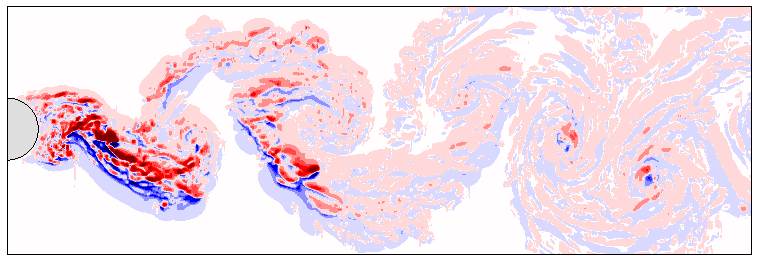
\includegraphics[width=\linewidth]{chapter5/a-posteriori/SR/SRy_lowres}
    \caption{$\mathcal{S}^R_y$} 
\end{subfigure}
\begin{subfigure}[t]{0.6\linewidth}
    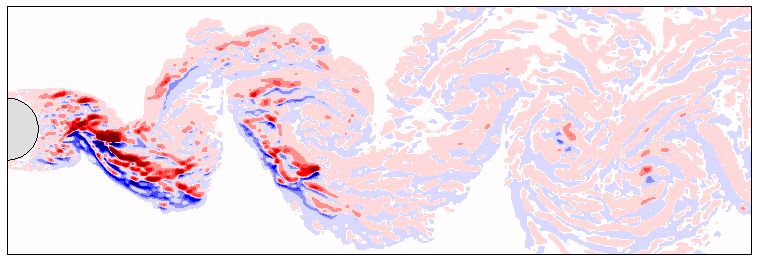
\includegraphics[width=\linewidth]{chapter5/a-posteriori/SR/SRy_ML_lowres}
    \caption{$\mathcal{S}^{R,\,\mathrm{ML}}_y$} 
\end{subfigure}
\caption{ML model prediction of the perfect closure components.}
\label{fig:ML_SR_a-priori}
\end{figure}

\begin{figure}[t]
\centering
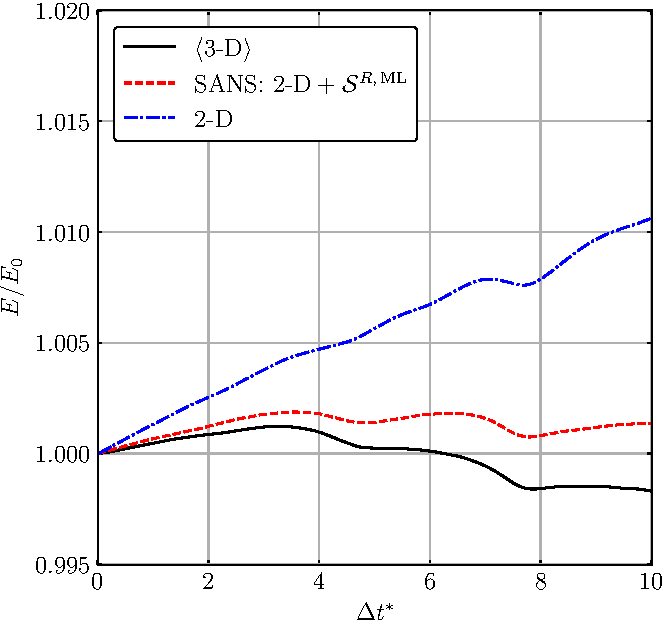
\includegraphics[width=0.50\linewidth]{chapter5/a-posteriori/E}
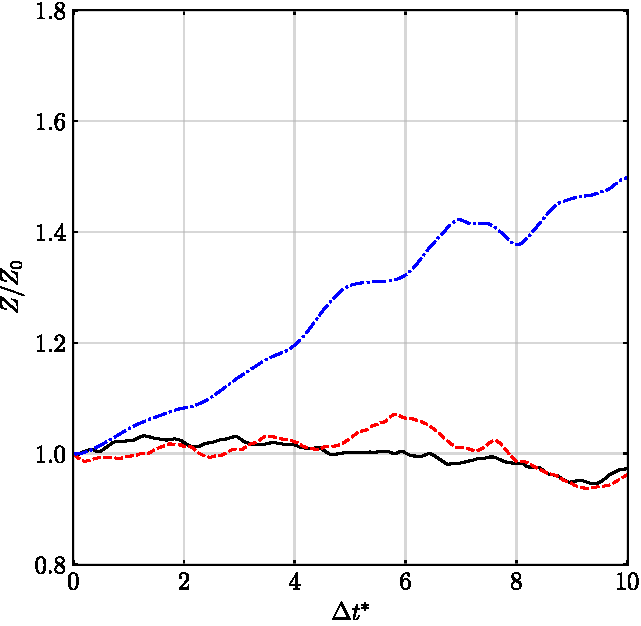
\includegraphics[width=0.48\linewidth]{chapter5/a-posteriori/Z}
\caption{Kinetic energy (left) and enstrophy (right) evolution during $\Delta t^*=10$ for the 3-D spanwise-averaged (reference data), SANS, and 2-D systems.
Simulations are started from a 3-D spanwise-averaged snapshot at $t^*_0$, corresponding to the scaling energy $(E_0)$ and enstrophy $(Z_0)$.
Energy and enstrophy are computed as detailed in \fref{fig:perfect_t-g} caption.}
\label{fig:E_Z_a-posteriori}
\end{figure}
\begin{figure}[t]
\centering
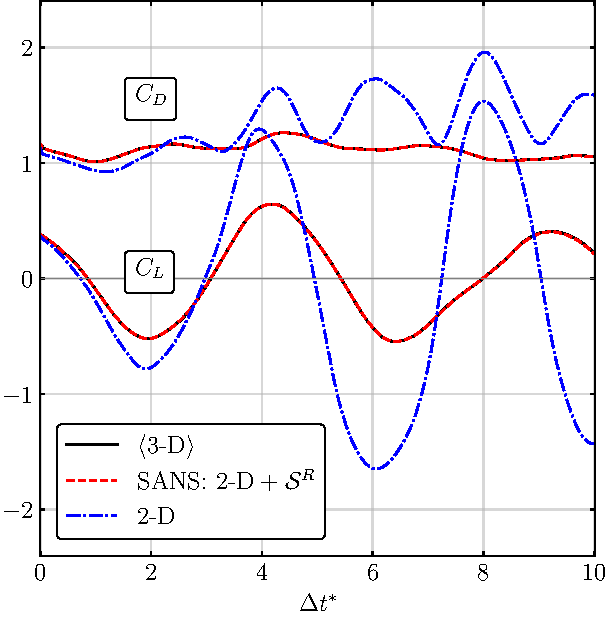
\includegraphics[width=0.48\linewidth]{chapter5/a-posteriori/forces}
\caption{Lift (bottom) and drag (top) forces induced to the cylinder (computed as described in \fref{fig:perfect_cc_forces}).
The lines legend is equivalent to \fref{fig:E_Z_a-posteriori}.}
\label{fig:forces_a-posteriori}
\end{figure}

Additionally, the instantaneous spanwise vorticity is depicted in \fref{fig:ML_a-posteriori}.
It is worth noting that the shear layer roll-up region of the SANS snapshot is not as coherent as the 2-D system, where structures have already reorganised into large scales.
In particular, the bottom detaching vortex of the SANS simulation is not as energised as the pure 2-D simulation one, and small-scale structures are still found in the SANS snapshot.
The close-wake region dictates the forces induced to the cylinder, explaining the significant difference in lift and drag forces shown in \tref{tab:ML_a-posteriori}.
In general, vortices found in the SANS simulation do not appear as coherent as in the 2-D case, where the inverse energy cascade promoted via vortex-merging and vortex-thinning events rapidly two-dimensionalises the wake structures.
A closer look on the SANS small-scale structures also shows that these are not correlated to the reference data.
This can also be appreciated at the top shear layer roll-up, where the error starts to propagate to the far field.
The ML closure error is responsible for such phenomenon, and ultimately yields the divergence of the system dynamics.

\begin{figure}[t]
\centering
\begin{subfigure}[t]{0.7\linewidth}
 	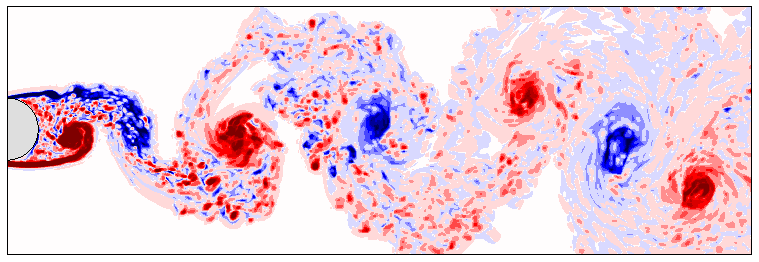
\includegraphics[width=\linewidth]{chapter5/a-posteriori/3-D_t=2651_lowres}
 	\caption{$\left\langle 3\text{-}\mathrm{D} \right\rangle$}
\end{subfigure}
\begin{subfigure}[t]{0.7\linewidth}
	\includegraphics[width=\linewidth]{chapter5/a-posteriori/SANS_t=2651_lowres}
	\caption{SANS}
\end{subfigure}
\begin{subfigure}[t]{0.7\linewidth}
	\includegraphics[width=\linewidth]{chapter5/a-posteriori/2-D_t=2651_lowres}
	\caption{$2\text{-}\mathrm{D}$}
\end{subfigure}
\caption{Spanwise vorticity snapshots for: (a) Spanwise-averaged 3-D flow (reference data).
(b) SANS with $\mathcal{S}^{R,\,\mathrm{ML}}$.
(c) 2-D simulation (no-model).
The SANS and the 2-D systems are started from a spanwise-averaged snapshot of the 3-D simulation at $t^*_0$.
The snapshots above correspond to $\Delta t^*=1$.}
\label{fig:ML_a-posteriori}
\end{figure}

\section{Discussion and conclusion}

This chapter introduces a ML model for the SANS equations, enabling 3-D turbulent flows with a homogeneous flow direction to be modelled using a 2-D system of equations with an observed speed up of 99.5\%.
The SSR tensor is critical to the success of this description, driving the 2-D flow dynamics to match the 3-D statistics and flow forces.
While EVMs are completely inadequate to model the SSR tensor, we develop a data-driven closure based on a deep-learning network with tested correlation statistics above 90\%.
The trained ML model also performs well in different Reynolds regimes and body geometries to the training case, despite some discrepancies in the near-body region.

The success of ML models for turbulent flows in an a-posteriori set-up is still limited, and the error propagation into the resolved quantities remains an open issue \citep{Wang2017, Beck2019}.
Stability has been previously achieved by projecting the ML model output into a known stable closure such as EVMs for time-averaged (RANS) or filtered (LES) systems \citep{Maulik2018, Beck2019, Cruz2019}.
Also, highly-resolved simulations help to mitigate the closure weight resulting in more stable computations \citep{Gamahara2017}.
Unfortunately, these solutions cannot be implemented in SANS because, as previously exposed, the EVMs hypothesis is intrinsically different from the nature of the SSR tensor.

Employing recurrent neural networks (RNN) for the prediction of SANS closure terms is a research direction worth exploring in the future.
RNNs incorporate the system temporal dynamics so they can offer a more stable a-posteriori solution targeting statistically stationary metrics \citep{Vlachas2018, Kim2020b}.
In this sense, the use of long-short term neural networks (a type of RNN) similarly to \cite{Vlachas2018}, together with CNNs could help overcome the issues exposed in the SANS closure.
Additionally, a physics-informed loss function can also improve the model stability as shown in \cite{Lee2019}.
Finally, while the current model is initialised from a 3-D averaged simulation, a more stable closure should be capable of developing 3-D turbulence dynamics even when initialised with a pure 2-D flow snapshot.

Overall, the new SANS flow description combined with advances in data-driven modelling has the potential to vastly improve the speed and accuracy of turbulence simulations for a prevalent class of engineering and environmental applications.
% ----------------------------------------------------------------
\end{document}
